\documentclass{sigchi-ext}
% Please be sure that you have the dependencies (i.e., additional
% LaTeX packages) to compile this example.
\usepackage[T1]{fontenc}
\usepackage{textcomp}
\usepackage[scaled=.92]{helvet} % for proper fonts
\usepackage{graphicx} % for EPS use the graphics package instead
\usepackage{balance}  % for useful for balancing the last columns
\usepackage{booktabs} % for pretty table rules
\usepackage{ccicons}  % for Creative Commons citation icons
\usepackage{ragged2e} % for tighter hyphenation

% Some optional stuff you might like/need.
% \usepackage{marginnote} 
% \usepackage[shortlabels]{enumitem}
% \usepackage{paralist}
% \usepackage[utf8]{inputenc} % for a UTF8 editor only

%% EXAMPLE BEGIN -- HOW TO OVERRIDE THE DEFAULT COPYRIGHT STRIP --
% \copyrightinfo{Permission to make digital or hard copies of all or
% part of this work for personal or classroom use is granted without
% fee provided that copies are not made or distributed for profit or
% commercial advantage and that copies bear this notice and the full
% citation on the first page. Copyrights for components of this work
% owned by others than ACM must be honored. Abstracting with credit is
% permitted. To copy otherwise, or republish, to post on servers or to
% redistribute to lists, requires prior specific permission and/or a
% fee. Request permissions from permissions@acm.org.\\
% {\emph{CHI'14}}, April 26--May 1, 2014, Toronto, Canada. \\
% Copyright \copyright~2014 ACM ISBN/14/04...\$15.00. \\
% DOI string from ACM form confirmation}
%% EXAMPLE END

% Paper metadata (use plain text, for PDF inclusion and later
% re-using, if desired).  Use \emtpyauthor when submitting for review
% so you remain anonymous.
\def\plaintitle{SIGCHI Extended Abstracts Sample File: Note Initial
  Caps} \def\plainauthor{First Author, Second Author, Third Author,
  Fourth Author, Fifth Author, Sixth Author}
\def\emptyauthor{}
\def\plainkeywords{Machine Learning; Codeblocks Programming; Novice Programmer Practices; Interactive Machine Learning}
\def\plaingeneralterms{Programming}

\title{TREX: A Visualization Tool For Linear Regression Experiments To Help Novice Programmers}

\numberofauthors{6}
% Notice how author names are alternately typesetted to appear ordered
% in 2-column format; i.e., the first 4 autors on the first column and
% the other 4 auhors on the second column. Actually, it's up to you to
% strictly adhere to this author notation.
\author{%
  \alignauthor{%
    \textbf{Jose Maria Santiago III}\\
    \affaddr{De La Salle University} \\
    \affaddr{2401 Taft Avenue, Malate, Manila, Philippines} \\
    \email{jose\_maria\_santiago@dlsu.edu.ph} }\alignauthor{%
    \textbf{}\\
    \affaddr{}\\
    \affaddr{}\\
    \email{} } \vfil \alignauthor{%
    \textbf{Giselle Nodalo}\\
    \affaddr{De La Salle University}\\
    \affaddr{2401 Taft Avenue, Malate, Manila, Philippines}\\
    \email{giselle\_nodalo@dlsu.edu.ph} }\alignauthor{%
    \textbf{}\\
    \affaddr{}\\
    \affaddr{}\\
    \email{} } \vfil \alignauthor{%
    \textbf{Jordan Aiko Deja}\\    
    \affaddr{De La Salle University} \\
    \affaddr{Manila, Philippines} \\
    \affaddr{University of Primorska} \\
    \affaddr{Koper, Slovenia} \\
    \email{jordan.deja@dlsu.edu.ph} }\alignauthor{%
    \textbf{}\\
    \affaddr{}\\
    \affaddr{}\\
    \affaddr{}\\
    \email{} } }

% Make sure hyperref comes last of your loaded packages, to give it a
% fighting chance of not being over-written, since its job is to
% redefine many LaTeX commands.
\definecolor{linkColor}{RGB}{6,125,233}
\hypersetup{%
  pdftitle={\plaintitle},
%  pdfauthor={\plainauthor},
  pdfauthor={\emptyauthor},
  pdfkeywords={\plainkeywords},
  bookmarksnumbered,
  pdfstartview={FitH},
  colorlinks,
  citecolor=black,
  filecolor=black,
  linkcolor=black,
  urlcolor=linkColor,
  breaklinks=true,
}

% \reversemarginpar%

\begin{document}

%% For the camera ready, use the commands provided by the ACM in the Permission Release Form.
%\CopyrightYear{2007}
%\setcopyright{rightsretained}
%\conferenceinfo{WOODSTOCK}{'97 El Paso, Texas USA}
%\isbn{0-12345-67-8/90/01}
%\doi{http://dx.doi.org/10.1145/2858036.2858119}
%% Then override the default copyright message with the \acmcopyright command.
%\copyrightinfo{\acmcopyright}

\begin{marginfigure}[3.0pc]
\begin{minipage}{\marginparwidth}
     \centering
    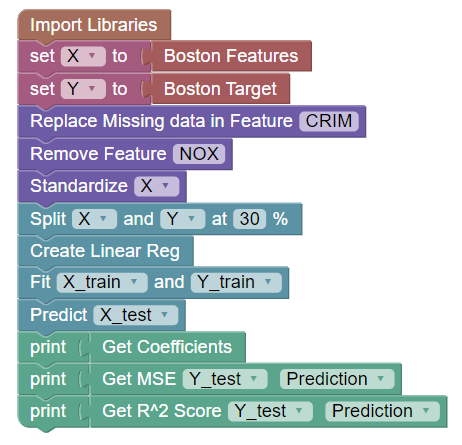
\includegraphics[width=4.5cm,height=4.5cm]{figures/IT3.png}
    \caption{Snippet of the codeblocks of the latest prototype. Codeblocks of the same function are colored and grouped together. }
    \label{fig:IT3_Blocks}
    \end{minipage}
\end{marginfigure}


\begin{marginfigure}[5pc]
\begin{minipage}{\marginparwidth}
     \centering
    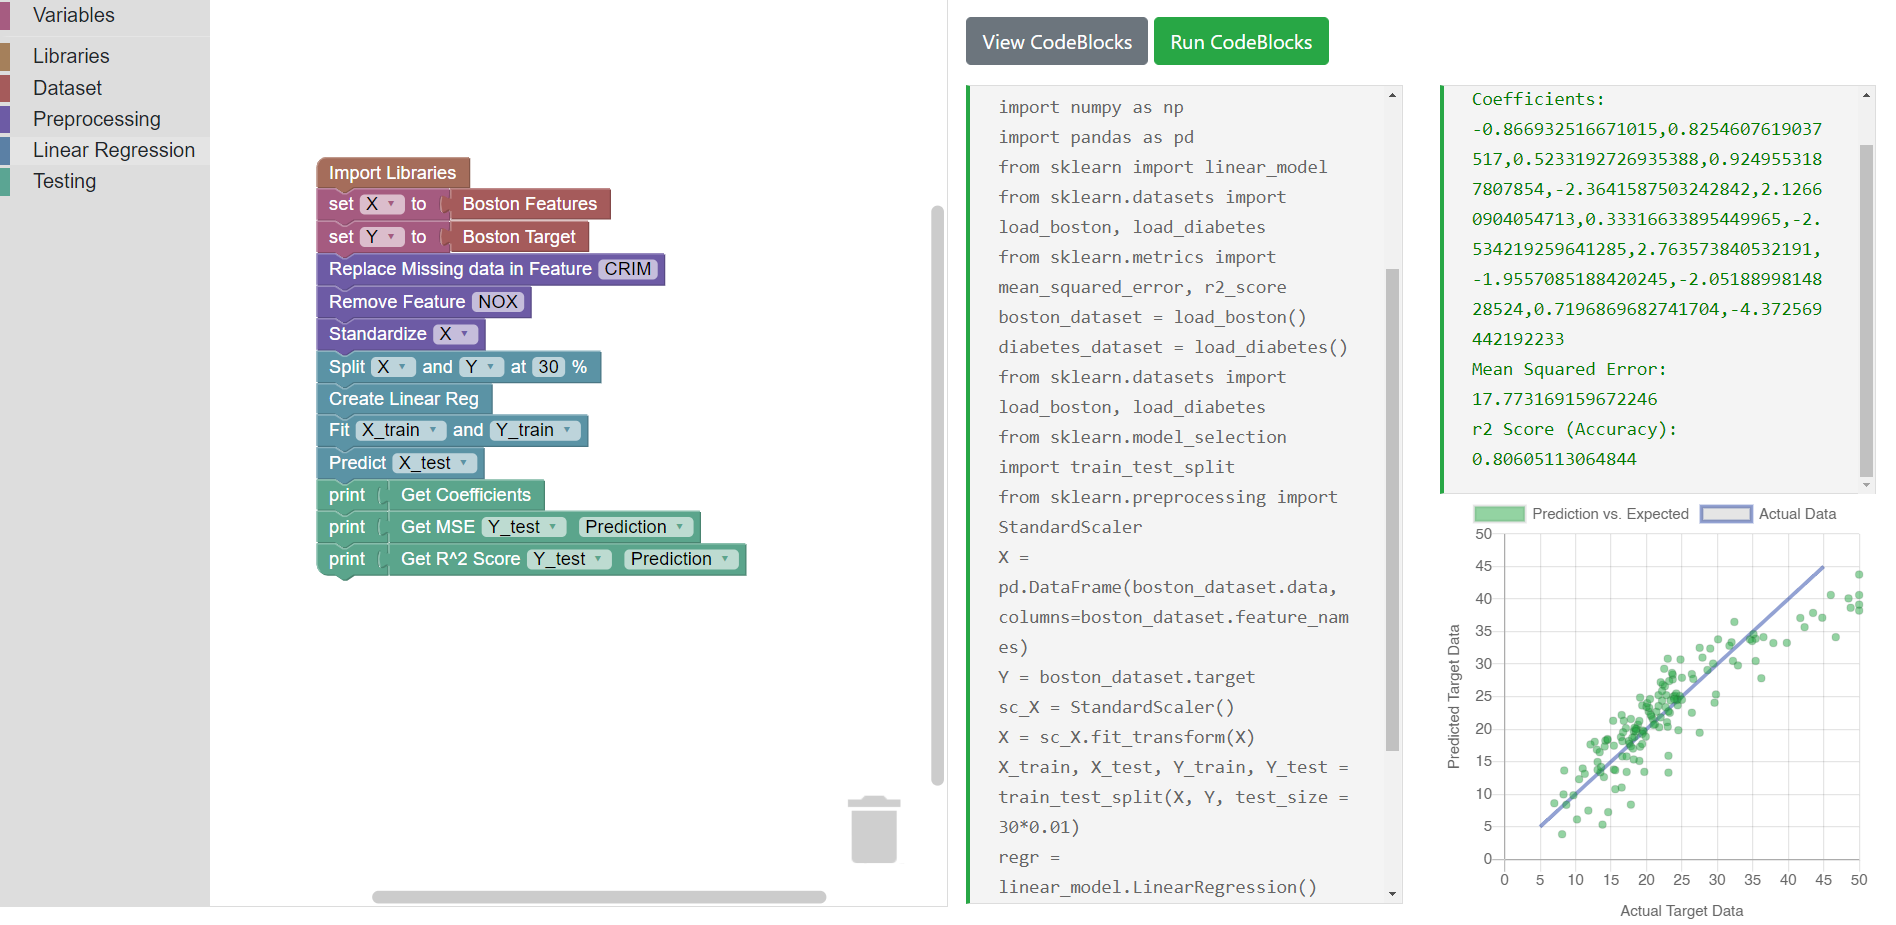
\includegraphics[width=4.75cm,height=3cm]{figures/Gen_Interface.png}
  \caption{A sample screenshot of the third prototype. The leftmost pane has a palette of block groups. The second left pane is a sandbox where they can drag and drop code blocks. The rightmost panes show the equivalent code. }
    \label{fig:prot3}
    \end{minipage}
\end{marginfigure}





\maketitle

% Uncomment to disable hyphenation (not recommended)
% https://twitter.com/anjirokhan/status/546046683331973120
\RaggedRight{} 

% Do not change the page size or page settings.
\begin{abstract}
  Machine Learning (ML) suites are readily-available for practical use. There are available packaged software and console libraries that can be modified. However, novice programmers avoid these ML suites due to the abstractions with pre-existing tools. Users with limited programming background that know how these models work, struggle with converting them to code for practical use. We iterated on developing a codeblocks tool for linear regression tasks where we did multiple usability tests involving at least 33 participants. We observed how they went through their ML tasks, and inquired into their pains and struggles in writing code. To help them in this learning process, we present TREX: A Tool for Regression Experiments, that allows novices in ML programming to gain more confidence with building code. 
\end{abstract}

% ACM Classfication

\begin{CCSXML}
<ccs2012>
<concept>
<concept_id>10003120.10003145.10011770</concept_id>
<concept_desc>Human-centered computing~Visualization design and evaluation methods</concept_desc>
<concept_significance>100</concept_significance>
</concept>
<concept>
<concept_id>10003120.10003121.10003122.10010854</concept_id>
<concept_desc>Human-centered computing~Usability testing</concept_desc>
<concept_significance>500</concept_significance>
</concept>
<concept>
<concept_id>10011007.10011074.10011092.10010876</concept_id>
<concept_desc>Software and its engineering~Software prototyping</concept_desc>
<concept_significance>500</concept_significance>
</concept>
<concept>
<concept_id>10003120.10003121.10003122.10003334</concept_id>
<concept_desc>Human-centered computing~User studies</concept_desc>
<concept_significance>300</concept_significance>
</concept>
</ccs2012>
\end{CCSXML}

\ccsdesc[500]{Human-centered computing~Human computer interaction (HCI)}
\ccsdesc[100]{Human-centered computing~User studies}
\ccsdesc[500]{Human-centered computing~Visualization design and evaluation methods}
\ccsdesc[100]{Software and its engineering~Software prototyping}

% Author Keywords
\keywords{\plainkeywords}

% Print the classficiation codes
\printccsdesc

\section{Introduction and Related Work}
Packaged Machine Learning (ML) programs such as WEKA and RapidMiner, were designed to enable novices to implement ML in projects without worrying about the code. However, users do not see the inner workings of a tool, often referred to as the blackbox effect. These users typically experience some issues when starting out. These users are either (1) computing professionals with adequate programming experience but lack the adequate foundation in ML or (2) professionals with preliminary knowledge on ML pipeline activities but lack adequate programming experience.

\begin{marginfigure}[-15pc]
\begin{minipage}{\marginparwidth}
     \centering
    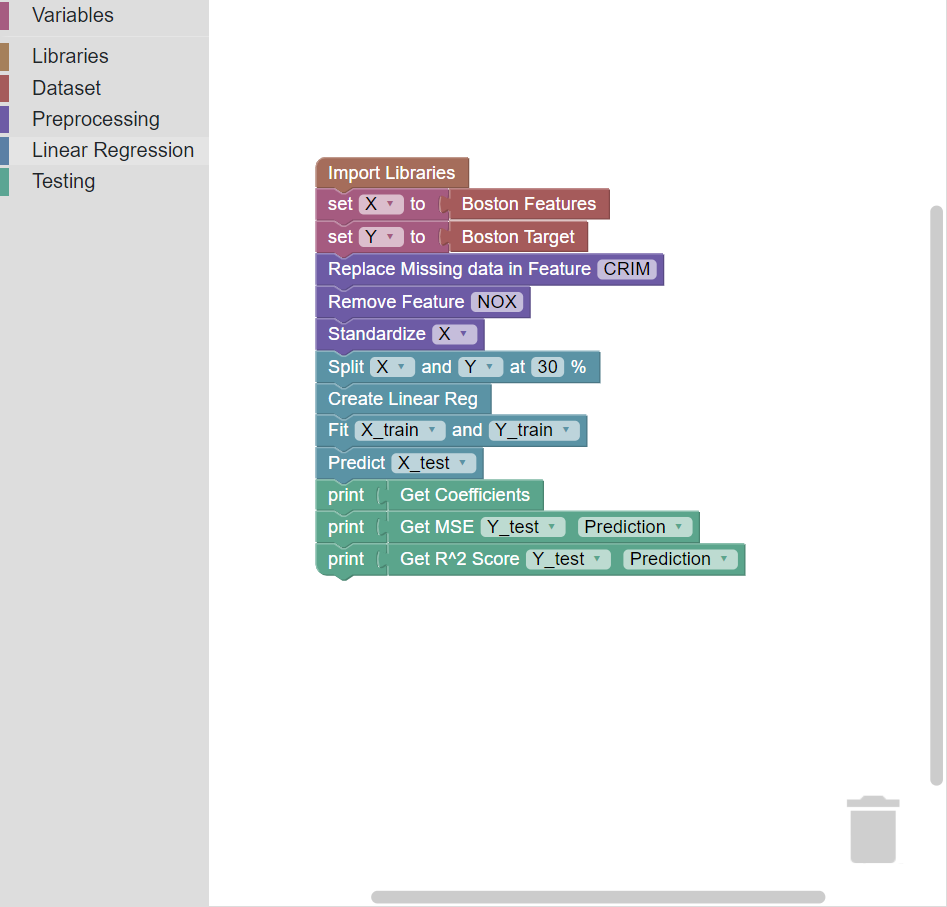
\includegraphics[width=4.5cm,height=4.65cm]{sigchi-latex-extended-abstracts/figures/codeblocks_categories.png}
    \caption{Snippet of the TREX Codeblocks and their categories}
    \label{fig:Code_cat}
    \end{minipage}
\end{marginfigure}

\begin{marginfigure}[1.5pc]
\begin{minipage}{\marginparwidth}
     \centering
    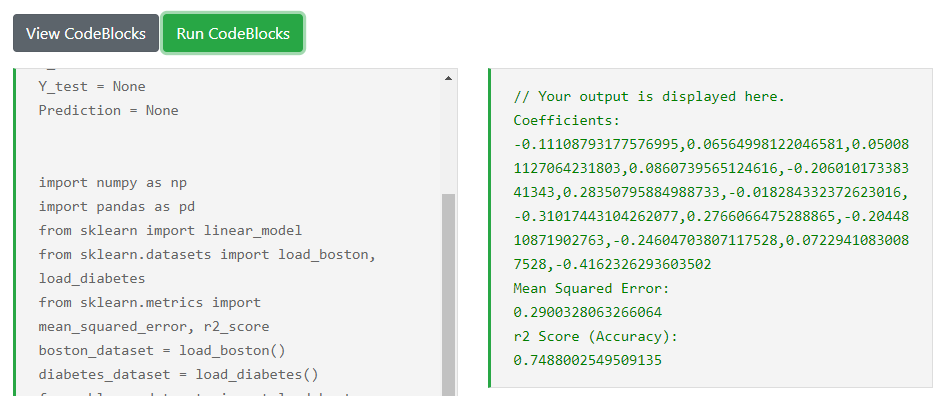
\includegraphics[width=4.5cm,height=2.5cm]{figures/Code_Output.png}
    \caption{Snippet of Code Output and Translation Section}
    \label{fig:Code_output}
    \end{minipage}
\end{marginfigure}

\begin{marginfigure}[1.5pc]
\begin{minipage}{\marginparwidth}
     \centering
    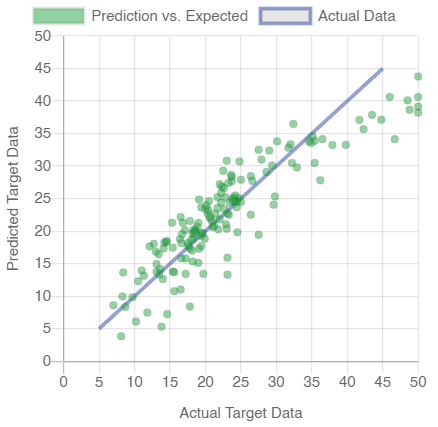
\includegraphics[width=4.5cm,height=4.5cm]{figures/Reg_Vis.png}
    \caption{The Sandbox Prototype Regression Visualization}
    \label{fig:Code_viz}
    \end{minipage}
\end{marginfigure}

A comparison done by \cite{nodalo2019building} found that visual tools, such as WEKA \& Rapidminer, are not entirely interactive. They provide limited user feedback and abstracts the algorithm code from the user. In the work of \cite{sarkar2015interactive}, novice ML students are exposed to ML while utilizing the interactive environment of spreadsheets. These platforms are often limited to their domain, such as finance and economics. Yet end-users easily understand how minor tweaking of formulas affect the output of these systems due to the familiarity of spreadsheet interactions. They also widen the range of ML practicality, allowing it to be expanded to other fields. The study of \cite{amershi2011designing,amershi2012regroup} investigates the use of an iML system that classified groups of people on social-networking sites to reduce the instance of unwanted data leaking to users. These systems give end-users an opportunity to work \& explore their experiments while considering specific constraints and ethical considerations. The works of \cite{das2019beames, zhao2019featureexplorer} attempted to design sandbox environments for regression experiments. They consider steering, inspection of ML but do not investigate on the activities and behaviors of the users themselves.


Tensorflow\footnote{https://tensorflow.org}, an open source ML framework that deals with high numerical computations, is designed to be easily accessible and for faster processing of ML algorithms, especially those that can be programmed with Tensors. TensorFlow Playground\footnote{https://playground.tensorflow.org} , is an exploratory sandbox that allows users to visualize how a Neural Network learns. The playground displays various components that users can tweak which also affects the output displayed on the interface. Algorithm Visualization (AV) is essential in improving a user's understanding of an algorithm's function \cite{shaffer2010algorithm}. The work of \cite{vrachnos2008dave} used dynamic AV that exposed novice learners to underlying algorithm logic. Platforms like this help fit the mental model of the user and their perceptions about the behavior of the algorithm itself. It has been observed that the programmers in agile settings consider factors that give them flexibility instead \cite{hussain2009current}. However, the study of \cite{sarkar2015interactive} observed users that often preferred a specific user flow as a result of using these iML systems, which were discovered from applying user-centered design processes in an agile setting. Ideally, this approach involving end-user innovation on iML systems states that the user centered design process can be applied to improve usability itself for novice users \cite{bernardo2016interactive} and systems targeted towards them. Several works have investigated on behaviors and productivity of programmers coming from different backgrounds and experiences. Our work investigates the underlying design factors that affect these behaviours. Attempting to understand the human factors involving novice users operating in an unfamiliar, block-based visual interface. In this paper we: (1) Observe \& understand how programmers implement code when given a linear regression task. We (2) discuss design implications for supporting the interaction needs of a novice user. Lastly, we (3) reflect on how we can design better interactive ML (iML) platforms that help novice-expert transitions in regression experiments.





%Learning algorithms have been made unified and interactive on web-based platforms as seen in the work of \cite{halim2012learning}. These improved the way novice learners absorbed algorithm lessons accompanied by appropriate scripted examples and animations. However, it is focused on visualizing data structures and non-ML algorithms.

\section{The TREX Tool}
\subsection{Participants and Methodology}
For creating TREX, the methodology used follows three (3) main phases as seen in figure \ref{fig:methodology}. The framework and prior user study used is a continuation of a previous study done in \cite{nodalo2019building} which follows an iterative approach. 
%In relation to this study, it involves designing and testing multiple versions of the Regression tool to improve previous iterations for novices based from their expectations and pain points. 
Novices for this study were undergraduate students from computing courses with basic knowledge of programming, and three (3) months to one (1) year experience with ML programming. A total of three (3) iterations were completed throughout the study accompanied by prior user research to aid with forming the features \& interactions to address pain points mentioned by potential novice users. All iterations were tested by novices who were gathered through purposive sampling. 

%\subsection{User Research}
%An initial user study was conducted through in-depth interviews with novice ML users that were familiar with different ML algorithms especially with programming Linear Regression. The participants were interviewed about their familiarity with ML concepts and the pain points they encounter while learning and using ML applications and libraries. The concept of code abstractions and code-blocks was briefly discussed with them to gain further insight of their expectations of the Regression tool. 

%Methodology Figure
\begin{marginfigure}[-2pc]
\begin{minipage}{\marginparwidth}
     \centering
    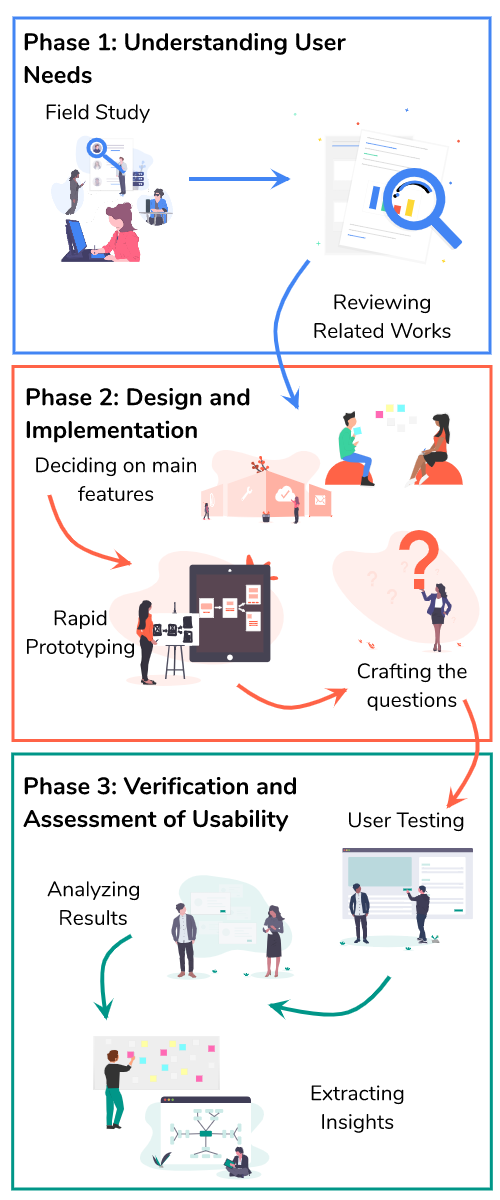
\includegraphics[width=4.5cm,height=12.5cm]{figures/Method-strip.png}
    \caption{Overview of the derived Research Framework, that follows a user-centric, and iterative approach based on the work of \protect\cite{nodalo2019building}. This user-centric approach involves ML novice programmers through each iteration of design and development of the tool.}
    \label{fig:methodology}
    \end{minipage}
\end{marginfigure}

\subsection{Iterative Prototyping With Code-block Abstractions}
%To design the prototype, insights gathered from prior user research were used to form user stories that were later converted into features for the tool. Following the interface structure of Scratch developed by \cite{mit:Scratch}, the tool was designed to have three sections \textemdash the code block work space, the code display, and a graph to visualize the model created. 
Initially, a prototype using static code blocks with similar naming conventions to Scikit-learn's library was created. Each category of code blocks were assigned specific colors to represent the phases of the ML pipeline. For the static prototype, three code block categories were prepared \textemdash Data Preprocessing, Linear Regression, and Test Model. An interactive prototype was later developed.
% using Google Blockly (the same code block technology used for Scratch),
% was used as the main interfacing blocks for the tool.
% the Scikit Learn Linear Regression library functions 
%for creating the Linear Regression model 
% and, Python's Django web framework allowed the tool to run code block generated Python code that is executed by the Python compiler. Additionally, Chart.js aided with creating an interactive scatter plot that updates as the model is updated. 
%Due to library limitations, additional code block categories were added to the iML prototype. These being Libraries (imports the necessary Python libraries), Variables (contains predefined variables), and Dataset (imports online datasets by Scikit-learn). 

\subsection{Usability Testing Codeblock Environment}
The prototypes were iteratively tested through usability testing. In the first iteration, each participant was tasked to map code blocks based on their understanding of the code samples provided. The second \& third iteration were done and tested using the main code environment of the tool. The second iteration was the initial interactive version which had no graphical visualization of the model but had the other basic features working. 
% Some insights from the first iteration were used to improve the code block design implemented for the second iteration. 
Participants were tasked to create Linear Regression systems with two datasets. The second iteration focused on discoverability to determine the common interactions participants follow when using the code blocks and when exposed to familiar programming environments such as using Google's Colaboratory. 
% Using improvement suggestions from the second iteration, 
In the third iteration prototype, four (4) tasks were given to the testers to explore the tool's features. A graphical visualization of the model was added to visualize the accuracy of the model. The focus of this iteration is to test the specific features of the iML tool and to observe how visualization of the model would influence the user. The experiment setup for each iteration can be seen in figure \ref{fig:setup}. This setup remained consistent for both the static (first iteration) and interactive (second and third iterations) prototypes tested. 
% The Participant was positioned in front of a laptop with the prototype available. The Facilitator was positioned beside the participant while tracking screen movement was recorded from the external monitor. The web camera of the desktop computer between the external monitor and the laptop was used to record the participants reactions and displayed the test flow and tasks. A voice recorder was used to record extra audio for the test. 
After each test, a System Usability Scale (SUS) survey and a word checklist was issued before conducting a short post-test interview to understand the participant's experience using the prototype. 

\subsection{TREX Features}
TREX is designed to be a web-based interactive tool that aims to provide the user with a sandbox environment for testing and creating Linear Regression ML Systems. All functions of the tool can be accessed in the dashboard which is separated into three sections as seen in figure \ref{fig:prot3}, each with a specific goal in mind. The three main sections are the Sandbox Environment section (figure \ref{fig:Code_cat}), Code Translationand Output section (figure \ref{fig:Code_output}), and the Regression Visualization section (figure \ref{fig:Code_viz}). TREX uses codeblocks which are connected to code segments similar to functions found in ML systems. We decided to create the system using a full-stack Python setup since we use Scikit-learn's Linear Regression library to run linear regression functions. This also provides easy-access to regression visualization libraries such as matplotlib for Python. When the system is compiled and run, the results are displayed on the output section of the dashboard. TREX uses the native error handling of the library along with custom error handling to address codeblock limitations such as incompatibility.

\section{Results}

Each iteration of the prototype was tested by at least five (5) to ten (10) ML users with varying skill levels, where two (2) of which identified themselves as novice users.
For iteration 1, all novices were intuitively following a pattern based on the ML Pipeline: Data Preprocessing, Model Training, and Model Testing. They were also consistent when ordering the Fit Data and Predict blocks. They placed the create-model block outside the model bracket which was designed to encompass the block. Novice users were observed to be experimental when using data preprocessing \& testing blocks. They found the tasks manageable. They also noted that organizing different ML phases by color made it easier, but were confused with the data preprocessing blocks. 


For iteration 2, most users enjoyed the block connecting sound. It reassures them of their progress and cited how the order of the blocks and categories follow the ML pipeline they identified. However, some users found the tool stressful causing them to skip tasks after misunderstanding how to use it, like stacking blocks horizontally rather than top to bottom. Some struggled figuring out the purpose of the ``Prediction'' block due to its colour being similar to the native Print block as seen in figure \ref{fig:IT2_Blocks}. Some users felt that the tool lacked flexibility when displaying outputs, and creating \& renaming variables while others wanted line numbers with proper error messages similar to traditional IDE's. The SUS survey score from this iteration was an average of 63.00 which falls into Grade D - Poor, seen in table \ref{tab:it2_sus}. This means the tool failed in terms of usability. This may be due to the types of errors participants encountered and their time adjusting and exploring the code blocks. 

\begin{marginfigure}[-45pc]
\begin{minipage}{\marginparwidth}
     \centering
    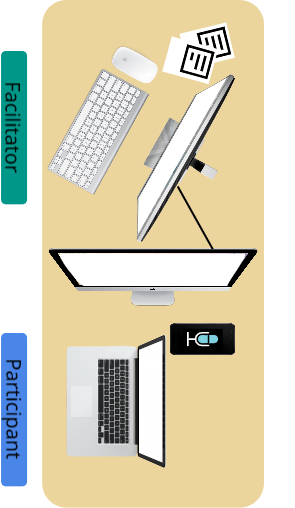
\includegraphics[width=4.5cm,height=6cm]{figures/setup.png}
    \caption{Test Setup for all usability testing of prototypes. The Participant was positioned in front of a laptop with the prototype available. The Facilitator was positioned beside the participant. Screen movement was recorded from the external monitor. The web camera of the desktop computer between the external monitor and the laptop was used to record the participant reactions and displayed the test tasks. A voice recorder was used to record extra audio for the test.}
    \label{fig:setup}
    \end{minipage}
\end{marginfigure}
\begin{marginfigure}[-8pc]
\begin{minipage}{\marginparwidth}
     \centering
    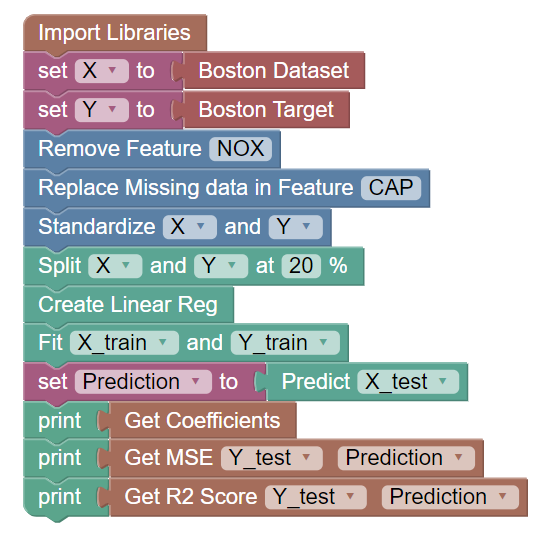
\includegraphics[width=4.5cm,height=4.5cm]{figures/IT2.png}
    \caption{Iteration 2 Code Blocks. As compared to Iteration 3 blocks, colors are not organized and sub parameters appear to be confusing.}
    \label{fig:IT2_Blocks}
    \end{minipage}
\end{marginfigure}

For iteration 3,
% three (3) ML users were selected for a beta version and another 
five (5) users were selected for the final version of the prototype.
% The beta version differs significantly with some of the colors, code block shapes, and error handling compared to the final version which was necessary as some errors were not fully resolved before moving to the final iteration.
Most users enjoyed using TREX code blocks to make base linear regression code due to its intuitiveness. However, some participants thought it was vague and frustrating to use due to misunderstanding the intent of error messages, which may lead to confusion. Due to the previous pain-point of connecting the ``Prediction'' block to the ``Print'' block, this lead to the design decision of hard-coding the initialization of the Prediction variable instead of maintaining the male jigsaw block shape that is similar in color to the native print block. The testing blocks for the final version of the prototype, as seen in figure \ref{fig:IT3_Blocks}, were also recoloured to green to be automatically associate them as output value blocks. The SUS survery score from this iteration received an average score of 80.50 which falls into a Grade A - Excellent, seen in table \ref{tab:it3_sus}. This means the tool is usable and functions towards user expectations. Between Iteration 2 and 3, there clearly is a significant increase in the SUS score from 63 to 80.50.



\section{Conclusion and Future Work}

As iML platforms are becoming more in demand, it is important to understand the human factors that influence the design of these systems. We designed and developed TREX: A Toolbox for Regression Experiments following the design methodology from \cite{nodalo2019building}. Through iterative prototyping and testing, we echo the findings of \cite{sarkar2015interactive}. Novice programmers tend to be less confident than their experienced counterparts. The behaviour they exhibited included: (1) exploring first their environment before building their solution as seen from our regression experiments (2) editing their existing code blocks based on their understanding of the ML pipeline, and finally (3) testing their assumptions and how it effects their model. With limited participants, our findings are yet to be verified through extensive testing. These findings emphasize the dynamic demand for better design in iML systems. With further research, we can still validate whether these behaviours are observable as well in other ML activities beyond regression experiments. 
\newpage
\begin{margintable}[1pc]
   \begin{minipage}{\marginparwidth}
     \centering
     \begin{tabular}{@{}cr@{}}
       \multicolumn{2}{r}{\textbf{Average Score for Iteration 2}} \\
       \midrule
       \textbf{Participant} & \multicolumn{1}{c}{\textbf{SUS Score}} \\ \midrule
        1 & 57.50 \\
        2 & 77.50 \\
        3 & 37.50 \\
        4 & 72.50 \\
        5 & 92.50 \\
        6 & 47.50 \\
        7 & 72.50 \\
        8 & 45.00 \\
        9 & 67.50 \\
        10 & 60.00 \\
        \begin{tabular}[c]{@{}c@{}}Average\end{tabular} & 63.00 \\
       \bottomrule
     \end{tabular}
     \caption{Average survey score for iteration 2 of the iML tool}
     \label{tab:it2_sus}
   \end{minipage}
 \end{margintable}
 
  \begin{margintable}[2.5pc]
   \begin{minipage}{\marginparwidth}
     \centering
     \begin{tabular}{@{}cr@{}}
    \multicolumn{2}{r}{\textbf{SUS Score for Iteration 3}} \\ \midrule
    \textbf{Participant} & \multicolumn{1}{c}{\textbf{SUS Score}} \\ \midrule
    1 & 85.00 \\
    2 & 85.00 \\
    3 & 85.00 \\
    4 & 72.50 \\
    5 & 75.00 \\
    \begin{tabular}[c]{@{}c@{}}Average\end{tabular} & 80.50 \\ \bottomrule
    \end{tabular}
     \caption{Average survey score for iteration 3 of the iML tool}
     \label{tab:it3_sus}
   \end{minipage}
 \end{margintable}

% \marginpar{%
%   \vspace{-45pt} \fbox{%
%     \begin{minipage}{0.925\marginparwidth}
%       \textbf{Good Utilization of the Side Bar} \\
%       \vspace{1pc} \textbf{Preparation:} Do not change the margin
%       dimensions and do not flow the margin text to the
%       next page. \\
%       \vspace{1pc} \textbf{Materials:} The margin box must not intrude
%       or overflow into the header or the footer, or the gutter space
%       between the margin paragraph and the main left column. The text
%       in this text box should remain the same size as the body
%       text. Use the \texttt{{\textbackslash}vspace{}} command to set
%       the margin
%       note's position. \\
%       \vspace{1pc} \textbf{Images \& Figures:} Practically anything
%       can be put in the margin if it fits. Use the
%       \texttt{{\textbackslash}marginparwidth} constant to set the
%       width of the figure, table, minipage, or whatever you are trying
%       to fit in this skinny space.
%     \end{minipage}}\label{sec:sidebar} }


\balance{} 
\bibliographystyle{SIGCHI-Reference-Format}

\bibliography{myreferences}


\end{document}

%%% Local Variables:
%%% mode: latex
%%% TeX-master: t
%%% End:
